% =========================================================================== %

\begin{frame}[t,plain]
\titlepage
\end{frame}

% =========================================================================== %

\begin{frame}{Script}
%
\begin{itemize}
\item Kapitel 16
	\begin{itemize}
	\item 16.1. Funktionen, die sich selbst aufrufen
	\item 16.2. Kommunikation über Rekursionsebenen hinweg 
	\item 16.4. Beispiel: Rekursives Auflisten der Ordnerstruktur
	\end{itemize}
\end{itemize}
%
\end{frame}

% =========================================================================== %

\begin{frame}[t,fragile]{Rekursion: Selbstaufrufe}
%
\begin{columns}[T]
\column{.75\linewidth}
\begin{itemize}
\item Routinen, die sich selbst aufrufen
\item Beispiel: Ordnerstruktur inklusive Unterordner durchsuchen
	\begin{itemize}
	\item alle Dateien des Stammverzeichnisses auflisten
	\item alle Ordner im Stammverzeichnis auflisten
	\item \emph{die Ordnerstruktur jedes Unterverzeichnisses auflisten}
	\item[$\Rightarrow$] Selbstbezug
	\end{itemize}
\item Manche Aufgaben so sehr elegant lösbar
\item Wartung schwierig
\end{itemize}
%
\begin{hintbox}
\footnotesize Um Rekursion zu verstehen, muss man zunächst Rekursion verstehen.
\end{hintbox}
%
\column{.2\linewidth}
\vspace{-10pt}
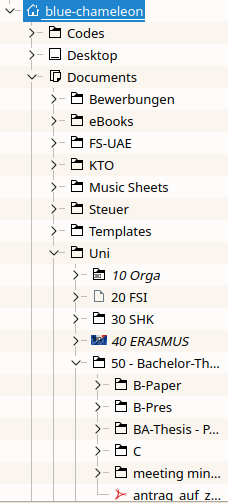
\includegraphics[width=\linewidth]{./gfx/foldertree}
%
\end{columns}
%
\end{frame}

% =========================================================================== %

\begin{frame}[fragile]{Ein einfacheres Beispiel: Summe einer Liste}
%
\begin{tcolorbox}
\emph{Die Summe aller Elemente einer Liste ist gleich dem ersten Listenelement plus der
Summe der verbleibenden Liste ohne ihr erstes Element.}
\end{tcolorbox}
%
\begin{itemize}
\item Rekursive Formulierung: Berechnung der Summe durch Kenntnis einer \emph{Untersumme}
\item Abbruchbedingung: \emph{triviale Liste}: Nur ein Element
\item Lehrbeispiel; Lösung über \mintinline{c}{for}-Schleife effizienter
\item So eine Lösung ist aber nicht immer verfügbar
\end{itemize}
%
\end{frame}

% =========================================================================== %

\begin{frame}[fragile]
%
\begin{codebox}[Code: Summe einer Liste]
\begin{minted}[fontsize=\scriptsize, linenos, firstnumber=last]{c}
#include <stdio.h>

int listsum_recursive(int * list, unsigned int N) {
  if (N == 1) {
    return list[0];
    
  } else {
    return list[0] + listsum_recursive(list + 1, N - 1);
  }
}

int main () {
  int list[] = {1, 2, 3, 4, 5, 6, 7, 8, 9};
  printf("Summe: %d\n", listsum_recursive(list, sizeof(list) / sizeof(*list)));
}

\end{minted}
\end{codebox}
%
\end{frame}

% =========================================================================== %

\begin{frame}
%
\tcbset{width=.7\linewidth, on line}
\scriptsize
\begin{codebox}[Rekursionsstufe 0: Symbol und Werte, equal height group=grRecIn]
\texttt{N = 9, list = \{1, 2, 3, 4, 5, 6, 7, 8, 9\}}
\begin{codebox}[Rekursionsstufe 1: Symbole und Werte]
\texttt{N = 8, list = \{2, 3, 4, 5, 6, 7, 8, 9\}}
\begin{codebox}[Rekursionsstufe 2: Symbole und Werte]
\texttt{N = 7, list = \{3, 4, 5, 6, 7, 8, 9\}}
\begin{codebox}[Rekursionsstufe 3-7]
...
\begin{codebox}[Rekursionsstufe 8]
\texttt{N = 1, list = \{9\}}%
\end{codebox}%
\end{codebox}%
\end{codebox}%
\end{codebox}%
\end{codebox}
%
\tcbset{width=.28\linewidth, on line}
\small
\begin{hintbox}[Beachte, equal height group=grRecIn]
Jeder Aufruf \enquote{lebt} in seinem eigenen Scope! Das Symbol \texttt{N} bezeichnet jeweils unterschiedliche Speicherstellen!

Dasselbe gilt für den \emph{Pointer} \texttt{list} (jedoch nicht für die Daten der Liste selbst).
\end{hintbox}
%
\end{frame}

% =========================================================================== %

\begin{frame}[fragile]
%
\begin{codebox}[Code: Summe einer Liste]
\begin{minted}[fontsize=\scriptsize, linenos, firstnumber=last]{c}
#include <stdio.h>

int listsum_recursive(int * list, unsigned int N) {
  if (N == 1) {
    return list[0];
    
  } else {
    return list[0] + listsum_recursive(list + 1, N - 1);
  }
}

int main () {
  int list[] = {1, 2, 3, 4, 5, 6, 7, 8, 9};
  printf("Summe: %d\n", listsum_recursive(list, sizeof(list) / sizeof(*list)));
}

\end{minted}
\end{codebox}
%
\end{frame}

% =========================================================================== %

\begin{frame}
%
\scriptsize
\begin{codebox}[Rekursionsstufe 0: Rückgabewerte]
\begin{codebox}[Rekursionsstufe 1: Rückgabewerte]
\begin{codebox}[Rekursionsstufe 2: Rückgabewerte]
\begin{codebox}[Rekursionsstufe 3-7]
\begin{codebox}[Rekursionsstufe 8: Rückgabewerte]
\texttt{return 9};
\end{codebox}
...
\end{codebox}
\texttt{return 3 + 39};
\end{codebox}
\texttt{return 2 + 42};
\end{codebox}
\texttt{return 1 + 44};
\end{codebox}
%
\end{frame}

% =========================================================================== %

\begin{frame}[t,fragile]%{Rekursion: Selbstaufrufe}
%
\tcbset{width=.6\linewidth, on line}
\begin{codebox}[Beispiel: Fakultät, equal height group = xmpFactorial]
\begin{minted}[fontsize=\scriptsize, linenos]{c}
#include <stdio.h>

int factorial (int n) {
    if (n > 1) {
        return n * factorial(n-1);
    } else if (n < 1) {
        printf("invalid argument\n"); 
        return -1;
    } else {
        return 1;
    }
}

int main(void) {
    for (int n=0; n<10; n++) {
        printf("%d! = %d\n", n, factorial(n));
    }
}
\end{minted}
\end{codebox}
%
\tcbset{width=.38\linewidth, on line}
\begin{hintbox}[Definition: Fakultät, equal height group = xmpFactorial]
\[N! = N \cdot (N-1) \cdot ... \cdot 1 \]
oder
\[N! = \prod_{i=1}^{N} i \]
\end{hintbox}
\end{frame}

% =========================================================================== %

\begin{frame}{Rekursion: Bemerkungen}
%
\begin{itemize}
\item Jeder rekursive Algorithmus in einfachen Schleifen darstellbar, und umgekehrt
\item Schleifen sind immer schneller
	\begin{itemize}
	\item Parameter auf Stack kopieren, Rücksprung-Punkt speichern, Springen und zurück kehren brauchen extra-Zeit
	\end{itemize}
\item Viele Algorithmen aber bedeutend leichter rekursiv formulierbar
	\begin{itemize}
	\item Rekursive Struktur vieler Probleme durch entsprechenden Code ausnutzbar
	\end{itemize}
\item Teilweise: Auflösung rekursiver Algorithmen vom Compiler
\item Schwerpunkt in der VL: \emph{Algorithmen und Datenstrukturen}\\
	(jedes Sommersemester, Dr. Stefan Solbrig)
\end{itemize}
%
\end{frame}

% =========================================================================== %

\begin{frame}{Beispiel: Mergesort}
%
\begin{itemize}
\item Ziel: Sortiere eine Liste von Werten
\item Zur Erinnerung: Bubblesort braucht $\mathcal{O}(N^2)$ Operationen (Vergleiche) für eine Liste mit $N$ Elementen\\
	\Thus Langsam für große Listen
\item Mergesort schafft das in $\mathcal{O}(N \log_2(N))$ Operationen\\
	\Thus Bedeutend schneller
\item Grundidee: 
	\begin{itemize}
	\item Aus zwei \emph{sortierten} Listen lässt sich schnell eine sortierte kombinierte Liste zusammenfügen (\emph{merge})
	\item Eine Liste mit mehr als einem Element lässt sich immer in zwei Teile teilen
	\item Eine Liste mit einem Element ist trivial sortiert
	\end{itemize}
\end{itemize}
%
\end{frame}

% =========================================================================== %

\begin{frame}[fragile]{Sorted Merge Step}
%
\begin{columns}
\column{.5\linewidth}
\begin{itemize}
\item Starte mit zwei \emph{sortierten} Listen
\item Wähle jeweils das erste Element jeder Liste als \emph{aktives Element}
\item Vergleiche die beiden aktiven Elemente
\item Füge das kleinere Element zur Ergebnis-Liste hinzu
\item Bei der Liste, aus der das kleinere Element stammte: rücke das aktive Element eins weiter
\item Wiederhole, bis alle Elemente verbraucht sind
\item[\Thus] Maximal $N$ Operationen
\end{itemize}
%
\column{.5\linewidth}
\begin{tcolorbox}
\begin{itemize}
\item \texttt{1, 4, 5, 8} und \texttt{2, 3, 6, 7}
\item \texttt{{\color{red} 1}, 4, 5, 8} und \texttt{{\color{red} 2}, 3, 6, 7}
\item \texttt{{\color{red} 1} < {\color{red}2}}
\item \texttt{\{1\}}
\item \texttt{1, {\color{red} 4}, 5, 8} und \texttt{{\color{red} 2}, 3, 6, 7}
\item \texttt{{\color{red} 4} > {\color{red}2}}
\item \texttt{\{1, 2\}}
\item \texttt{1, {\color{red} 4}, 5, 8} und \texttt{2, {\color{red} 3}, 6, 7}
\item ...
\item \texttt{\{1, 2, 3, 4, 5, 6, 7, 8\}}
\end{itemize}
\end{tcolorbox}
\end{columns}
%
\end{frame}

% =========================================================================== %

\begin{frame}{Prinzip Rekursiv Anwenden}
%
\vspace{-5pt}
\begin{columns}[T]
\column{.45\linewidth}
\begin{itemize}
\item Listen so lange halbieren, bis man sortierte Sublisten findet (spätestens bei Länge 1)
\item Meist: \emph{Immer} bis Länge 1
\item Sortierte Listen \emph{paarweise} nach vorgestelltem Prinzip zusammenfügen
\item Größere Listen ebenfalls zusammenfügen
\item Fertig!
\item Liste muss \emph{nicht} Länge $2^k$ haben!
\end{itemize}
%
\column{.55\linewidth}
\vspace{-7pt}
\begin{tcolorbox}
\begin{center}
\texttt{\{1,8,2,7,6,3,5,4\}} \\
$\Downarrow$ \\
\texttt{\{1,8,2,7\}} ~ \texttt{\{6,3,5,4\}} \\
$\Downarrow$ \\
\texttt{\{1,8\}} \texttt{\{2,7\}} \quad \texttt{\{6,3\}} \texttt{\{5,4\}} \\
$\Downarrow$ \\
\texttt{\{1\}} \texttt{\{8\}} ~
\texttt{\{2\}} \texttt{\{7\}} \quad
\texttt{\{6\}} \texttt{\{3\}} ~
\texttt{\{5\}} \texttt{\{4\}} \\
$\Downarrow$ \\
\texttt{\{1,8\}} \texttt{\{2,7\}} \quad \texttt{\{3,6\}} \texttt{\{4,5\}} \\
$\Downarrow$ \\
\texttt{\{1,2,7,8\}} \texttt{\{3,4,5,6\}} \\
$\Downarrow$ \\
\texttt{\{1,2,3,4,5,6,7,8\}}
\end{center}
\end{tcolorbox}
\end{columns}
%
\end{frame}

% =========================================================================== %

\begin{frame}
%
\begin{center}
Code Mergesort...
\end{center}
%
\end{frame}